\section{Algorithm}
\label{sec:algorithm}

Our algorithm is a multi-step process that identifies the bounding box of the item and then use homography transform to produce the final image.
We will now walk through the algorithm with a sample image seen in figure~\ref{fig:normal}.

\begin{figure}[t]
\begin{center}
   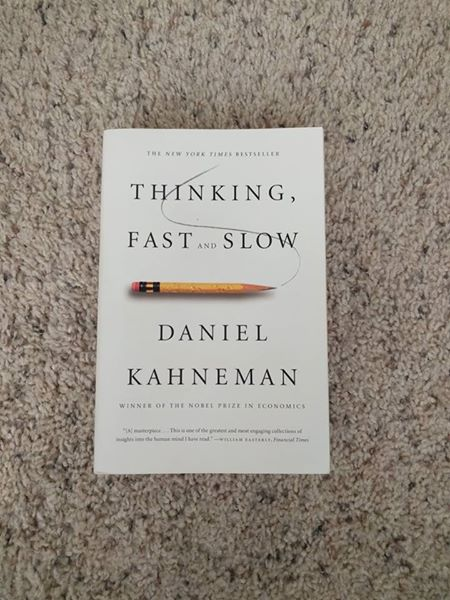
\includegraphics[width=0.8\linewidth]{figures/normal.jpg}
\end{center}
\caption{What the image looks like before any modification.}
\label{fig:normal}
\end{figure}

The first step of the algorithm is to identify edges in the image.
We converted the images to gray scale.
Then we smooth the image with a gaussian filter to help remove some background noise.
Then we use a canny edge detector to give us the binary image of edges.
Because of the non-maximal supression the canny edge detector, it gives us the best chance of getting fine lines.
Fine lines enable the next steps in our algorithm to be more precise.
The output of the edge dection can be seen in figure~\ref{fig:edge}.

\begin{figure}[t]
\begin{center}
   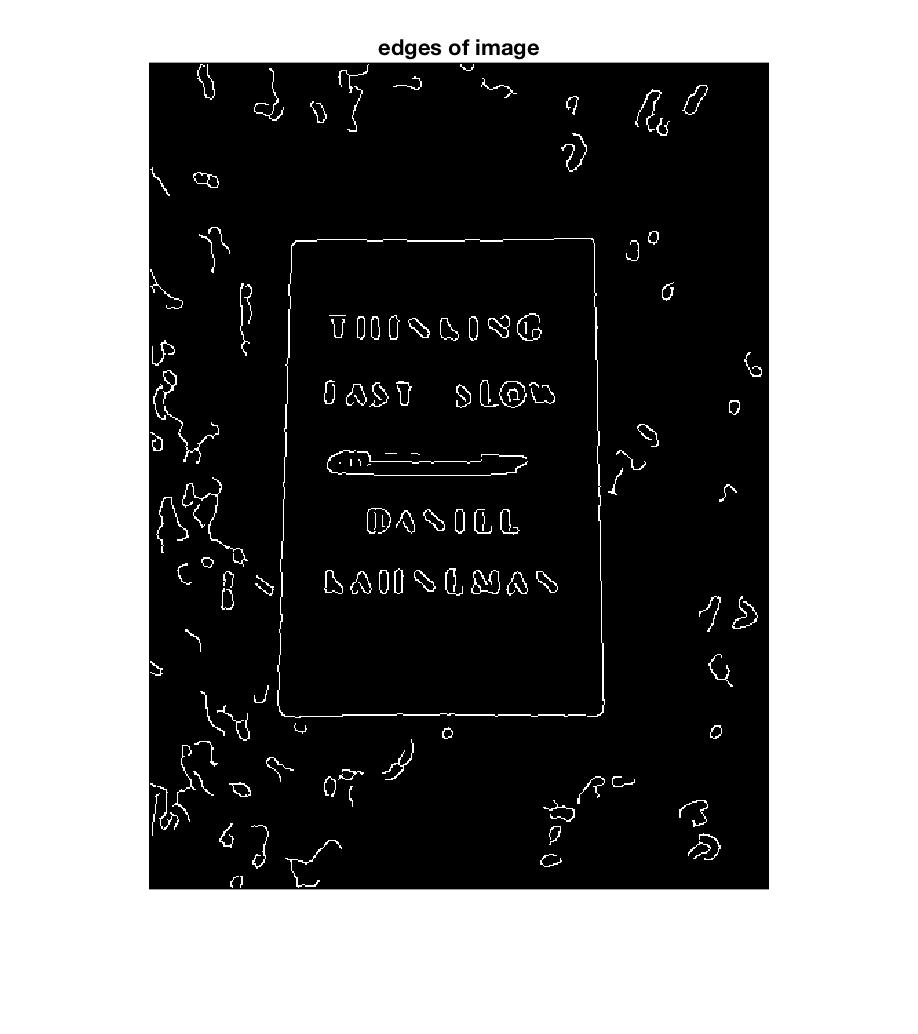
\includegraphics[width=0.8\linewidth]{figures/edgeDetection.jpg}
\end{center}
\caption{After edge-detection.}
\label{fig:edge}
\end{figure}

Once we have the binary image of edges we need to detect which edges correspond to straight lines.
To accomplish this we use the Hough transform~\cite{hough}.
Hough transform indentifies lines by keeping track of the pixels in terms of their slope.
If a bunch of pixel belongs to a line, they should have the similar slope with respect to a starting point.
The Hough transform algorithm keep track and score the collection of pixels.
We set this transformation such that gives us up to 10 line candidates.
These prospective lines can be seen in figure~\ref{fig:lines}

\begin{figure}[t]
\begin{center}
   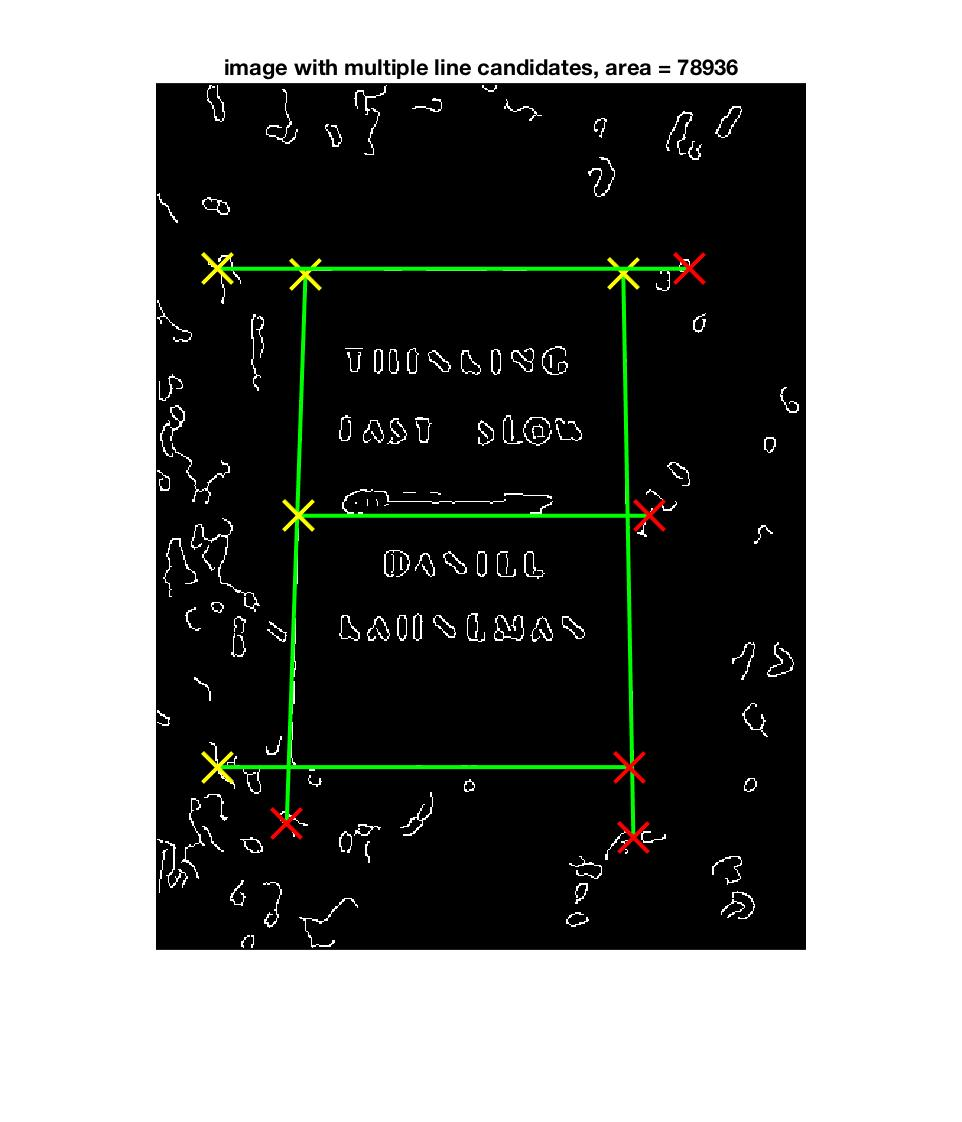
\includegraphics[width=0.8\linewidth]{figures/step2.jpg}
\end{center}
\caption{The second step}
\label{fig:lines}
\end{figure}

Next we use a random sampling method inspired by RANSAC to pick the lines that best represent the item.
In this step we use some assumptions about the images to develop a heuristic for which lines should be best.
Hough transform returns the coordinates of the endpoints of the lines.
From there, we can compute the vector that parametrizes the line.
To determine the corner, which is the intersection of a horizontal and vertical line, we perform cross product on the vectors of the lines.
We assume that the largest quadrilateral in the image is the item, such that maximizing the area of our polygon will be the correct bounding box for our item.
We also assume that it will be approximately rectangular, such that lines forming near right angles are preferred over acute or obtuse angles.
Using this criteria we then randomly sample four lines from the set keeping track of which best meets our heuristic.
At the end of this process we have four lines we believe to lie on the bounding box of the item.
With these lines we then find their intersections and mark these as the corners of the item.
The result of this step can be seen in figure~\ref{fig:box}.


\begin{figure}[t]
\begin{center}
   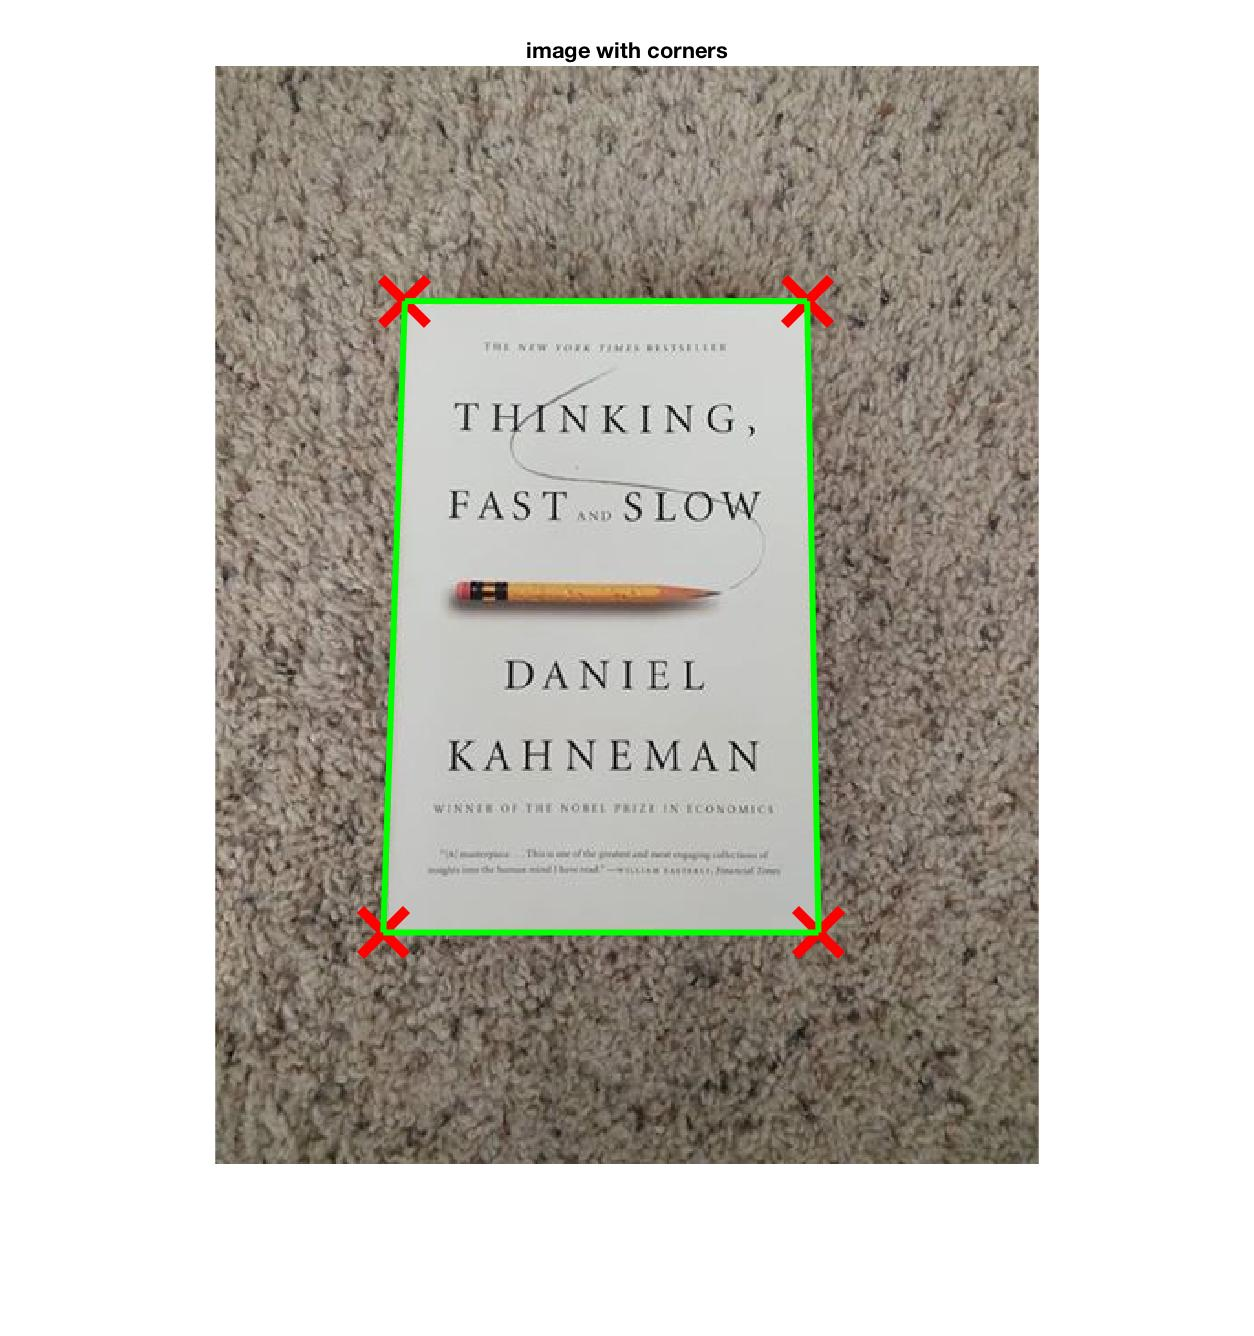
\includegraphics[width=0.8\linewidth]{figures/step3.jpg}
\end{center}
\caption{The third step}
\label{fig:box}
\end{figure}

Finally we use this set of corners as the input to a homography transformation.
Once we have computed the transform we then transform all pixels in the bounding box to get the final image as seen in figure~\ref{fig:final}.


\begin{figure}[t]
\begin{center}
   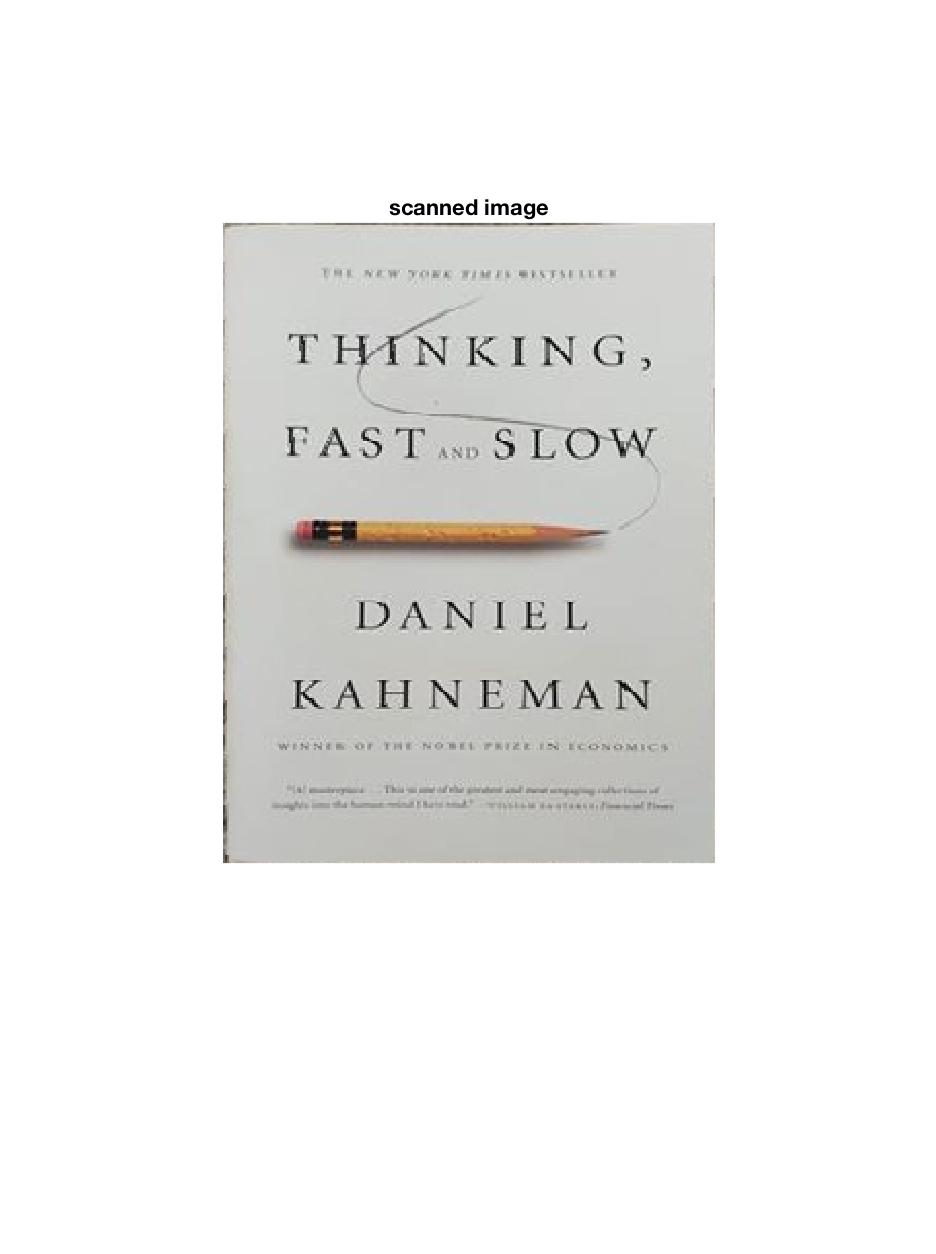
\includegraphics[width=0.8\linewidth]{figures/step4.jpg}
\end{center}
\caption{The fourth step}
\label{fig:final}
\end{figure}
